\documentclass[aspectratio=169,xcolor=dvipsnames]{beamer}

% Modern colorful theme
\usetheme{Madrid}
\usecolortheme{seahorse}

% Custom colors from original thesis
\definecolor{cwAlert}{RGB}{220,50,50}
\definecolor{cwFlow}{RGB}{50,120,220}
\definecolor{cwDecoy}{RGB}{120,180,50}
\definecolor{cwBorder}{RGB}{80,80,80}
\definecolor{ImperialBlue}{RGB}{0,62,116}
\definecolor{ImperialNavy}{RGB}{0,33,71}
\definecolor{ImperialLightBlue}{RGB}{155,203,235}

% Set theme colors
\setbeamercolor{structure}{fg=ImperialBlue}
\setbeamercolor{palette primary}{bg=ImperialNavy,fg=white}
\setbeamercolor{palette secondary}{bg=ImperialBlue,fg=white}
\setbeamercolor{palette tertiary}{bg=ImperialLightBlue,fg=ImperialNavy}
\setbeamercolor{frametitle}{bg=ImperialBlue,fg=white}
\setbeamercolor{title}{fg=ImperialNavy}

% Packages
\usepackage{tikz}
\usepackage{amsmath}
\usepackage{amssymb}
\usepackage{booktabs}
\usepackage{adjustbox}
\usepackage{xcolor}
\usepackage{colortbl}
\usepackage{pgfplots}
\pgfplotsset{compat=1.18}
\usetikzlibrary{shapes,arrows,positioning,shadows,patterns}
\usetikzlibrary{shapes,arrows,positioning,shadows,patterns}
\usetikzlibrary{arrows.meta} 

% Title information
\title[Adaptive Cyber Defense with AI]{\textbf{Adaptive Resource Placement for Cyber Defense}}
\subtitle{\textbf{Better Protection Through Multi-Agent Reinforcement Learning}}
%89\%
\author[M. Akanmode]{Miracle Akanmode}
\institute[Imperial College London]{
    Department of Computing\\
    Imperial College London\\
    \vspace{0.2cm}
    Supervisor: Kelly Zhang
}
\date{September 2025}

\begin{document}

%----------------------------------------------------------------------
% TITLE SLIDE
%----------------------------------------------------------------------
\begin{frame}
\vspace{0.25cm}
% Logo in top left
\begin{flushleft}

\includegraphics[height=0.7cm]{/rds/general/user/moa324/home/projects/cyberwheel/research_docs/poster/Images/ICL_Logo_Blue_RGB.pdf}
\end{flushleft}

\vspace{0.3cm}
\begin{center}
{\LARGE\textbf{\textcolor{ImperialNavy}{Adaptive Resource Placement}}}\\[0.12cm]
{\LARGE\textbf{\textcolor{ImperialNavy}{for Cyber Defense}}}\\[0.28cm]

{\large\textcolor{ImperialBlue}{Better Protection Through}}\\[0.08cm]
{\large\textcolor{ImperialBlue}{Multi-Agent Reinforcement Learning}}\\[0.4cm]
{\large\textbf{Miracle Akanmode}}\\[0.06cm]
{\normalsize Imperial-X}\\[0.07cm]
{\normalsize Imperial College London}\\[0.06cm]
\end{center}

\vfill
\begin{columns}[t]
    \column{0.5\textwidth}
    \begin{flushleft}
        {\normalsize Project Defense: September 2025}\\[0.06cm]
        {\normalsize Supervisor: Kelly Zhang}\\%[0.3cm]
    \end{flushleft}
        
    \column{0.5\textwidth}
    \begin{flushright}
        {\small\textcolor{ImperialBlue}{miracle.akanmode24@imperial.ac.uk}}
    \end{flushright}
\end{columns}
\vspace{1mm}
\end{frame}

%----------------------------------------------------------------------
% RESEARCH OVERVIEW
%----------------------------------------------------------------------
\begin{frame}{Research Overview}
\begin{columns}[c]
\column{0.6\textwidth}
\begin{itemize}
    \item \textbf{\textcolor{cwAlert}{Problem}}: Static cyber defenses fail against adaptive adversaries
    \item \textbf{\textcolor{cwFlow}{Approach}}: Multi-agent reinforcement learning for adaptive deception
    \item \textbf{\textcolor{cwDecoy}{Solution}}: PPO-based agent learning optimal honeypot placement
    \item \textbf{\textcolor{ImperialBlue}{Result}}: \textbf{89\% performance improvement} over baselines
\end{itemize}

\column{0.4\textwidth}
\begin{center}
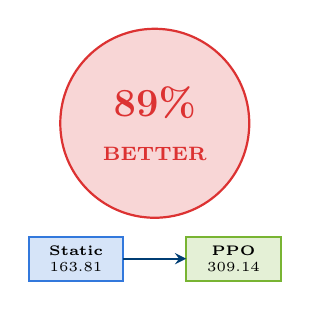
\begin{tikzpicture}[scale=0.8]
    \draw[fill=cwAlert!20, draw=cwAlert, thick] (0,0) circle (1.5);
    \node[align=center, font=\Large\bfseries] at (0,0) {\textcolor{cwAlert}{89\%}\\[-2pt]\textcolor{cwAlert}{\scriptsize BETTER}};
    
    \draw[fill=cwFlow!20, draw=cwFlow, thick] (-2,-2.5) rectangle (-0.5,-1.8);
    \node[align=center, font=\tiny] at (-1.25,-2.15) {\textbf{Static}\\163.81};
    
    \draw[fill=cwDecoy!20, draw=cwDecoy, thick] (0.5,-2.5) rectangle (2,-1.8);
    \node[align=center, font=\tiny] at (1.25,-2.15) {\textbf{PPO}\\309.14};
    
    \draw[-stealth, thick, ImperialBlue] (-0.5,-2.15) -- (0.5,-2.15);
\end{tikzpicture}
\end{center}
\end{columns}
\end{frame}

% ---------------------------------------------------------------------
% Quotes
% ---------------------------------------------------------------------
\begin{frame}{Ancient War Strategy Quotes}
\begin{block}{Sun Tzu Quotes}
\small
\begin{itemize}
  \item ``All warfare is based on deception.''
  \item ``He will win who knows when to fight and when not to fight.''
  \item ``The greatest victory is that which requires no battle.'' --- Sun Tzu, The Art of War.
\end{itemize}
\end{block}

\vspace{6pt}
\small These quotes support our approach: creating uncertainty and choosing when to act are central to the defense agent's strategy.
\end{frame}


%----------------------------------------------------------------------
% KEY TERMS & CONCEPTS  
%----------------------------------------------------------------------

\begin{frame}{Key Terms \& Concepts}
\small
\begin{columns}[t]
  \column{0.48\textwidth}
  \begin{description}[leftmargin=!,labelwidth=2.8cm]
    \item[\textbf{Reinforcement Learning}] Learning by trial and reward feedback.
    \item[\textbf{Agent}] The automated decision-maker (here: Blue agent).
    \item[\textbf{Environment}] The simulated network in which agents act.
    \item[\textbf{Policy}] Mapping from what the agent sees to actions.
    \item[\textbf{Reward}] Numeric signal that guides learning (good/bad).
  \end{description}

  \column{0.48\textwidth}
  \begin{description}[leftmargin=!,labelwidth=2.8cm]
    \item[\textbf{PPO}] A stable policy-optimisation algorithm used here.
    \item[\textbf{Action}] What the agent does (deploy/remove/wait).
    \item[\textbf{Observation / State}] What the agent perceives about the network.
    \item[\textbf{Honeypot / Decoy}] Fake asset used to lure and study attackers.
    \item[\textbf{Red / Blue Team}] Red = attacker (fixed); Blue = defender (learning).
  \end{description}
\end{columns}

\vspace{4pt}
\small Additional: MITRE ATT\&CK = standardised attacker techniques; "deception" = deliberate uncertainty creation to mislead attackers.
\end{frame}

%----------------------------------------------------------------------
% THE PROBLEM
%----------------------------------------------------------------------
\begin{frame}{The Cybersecurity Challenge}
\begin{columns}[c]
\column{0.5\textwidth}
\textbf{\textcolor{cwAlert}{Critical Challenges:}}
\begin{itemize}
    \item \textbf{Alert Fatigue}: 4,000+ daily alerts, 67\% ignored
    \item \textbf{Asymmetric Warfare}: Attackers need one success
    \item \textbf{Static Defenses}: Predictable patterns exploited
    \item \textbf{Base-Rate Fallacy}: Real threats missed
\end{itemize}

\column{0.5\textwidth}
\begin{center}
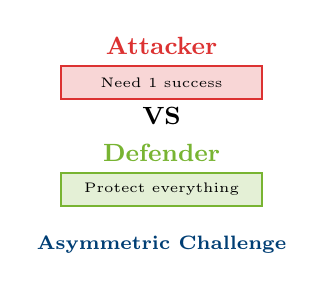
\begin{tikzpicture}[scale=0.85]
    % Attacker side (top)
    \node[font=\small\bfseries] at (1.5,2.3) {\textcolor{cwAlert}{Attacker}};
    \draw[fill=cwAlert!20, draw=cwAlert, thick] (0,2) rectangle (3,1.5);
    \node[align=center, font=\tiny] at (1.5,1.75) {Need 1 success};
    
    % VS in middle
    \node[font=\small\bfseries] at (1.5,1.25) {VS};
    
    % Defender side (bottom)
    \node[font=\small\bfseries] at (1.5,0.7) {\textcolor{cwDecoy}{Defender}};
    \draw[fill=cwDecoy!20, draw=cwDecoy, thick] (0,0.4) rectangle (3,-0.1);
    \node[align=center, font=\tiny] at (1.5,0.15) {Protect everything};
    
    % Asymmetric indicator
    \node[below, font=\scriptsize\bfseries] at (1.5,-0.4) {\textcolor{ImperialBlue}{Asymmetric Challenge}};
\end{tikzpicture}
\end{center}
\end{columns}

\vspace{0.5cm}
\begin{alertblock}{Our Solution}
\textbf{Adaptive AI-driven deception} that creates uncertainty for attackers through learned strategic honeypot placement
\end{alertblock}
\end{frame}


%----------------------------------------------------------------------
% DEFENSE EVOLUTION - EXACT TIKZ FROM ORIGINAL
%----------------------------------------------------------------------
\begin{frame}{Evolution of Cyber Defense}
\begin{center}
\scalebox{0.7}{
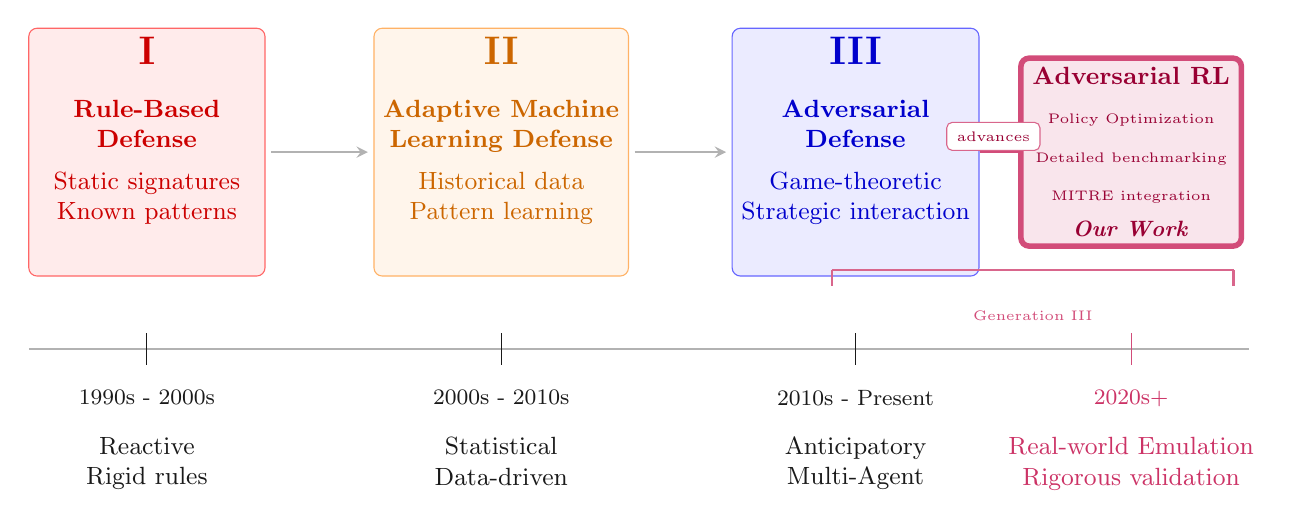
\begin{tikzpicture}[
    font=\small,
    generation/.style={
        draw=gray!40,
        fill=white,
        minimum width=3cm,
        minimum height=2.5cm,
        rounded corners=3pt,
        align=center
    },
    redaccent/.style={
        draw=red!60,
        fill=red!8,
        text=red!80!black
    },
    orangeaccent/.style={
        draw=orange!60,
        fill=orange!8,
        text=orange!80!black
    },
    blueaccent/.style={
        draw=blue!60,
        fill=blue!8,
        text=blue!80!black
    },
    ourwork/.style={
        draw=purple!70,
        fill=purple!10,
        minimum width=2.8cm,
        minimum height=2.3cm,
        rounded corners=3pt,
        align=center,
        line width=2pt,
        text=purple!80!black
    },
    arrow/.style={
        -stealth,
        thick,
        gray!60,
        shorten >=2pt,
        shorten <=2pt
    }
]
% Generation 1
\node[generation, redaccent] at (0,0) (g1) {
    {\Large \textbf{I}}\\[8pt]
    \textbf{Rule-Based}\\
    \textbf{Defense}\\[4pt]
    \small Static signatures\\
    \small Known patterns\\[6pt]
};
% Generation 2  
\node[generation, orangeaccent] at (4.5,0) (g2) {
    {\Large \textbf{II}}\\[8pt]
    \textbf{Adaptive Machine}\\
    \textbf{Learning Defense}\\[4pt]
    \small Historical data\\
    \small Pattern learning\\[6pt]
};
% Generation 3 - Updated to Adversarial
\node[generation, blueaccent] at (9,0) (g3) {
    {\Large \textbf{III}}\\[8pt]
    \textbf{Adversarial}\\
    \textbf{Defense}\\[4pt]
    \small Game-theoretic\\
    \small Strategic interaction\\[6pt]
};
% Our Work - Advanced approach within Gen 3
\node[ourwork] at (12.5,0) (ourwork) {
    \textbf{Adversarial RL}\\[3pt]
    \tiny  Policy Optimization\\[3pt]
    \tiny Detailed benchmarking\\[3pt]
    \tiny MITRE integration\\[2pt]
    \footnotesize \textbf{\textit{Our Work}}
};
% Evolution arrows
\draw[arrow] (g1.east) -- (g2.west);
\draw[arrow] (g2.east) -- (g3.west);
% Connection to our work (different style to show it's within Gen 3)
\draw[purple!70, thick] (g3.east) -- (ourwork.west);

% "Advances" in its own small box with text wrapping
\node[draw=purple!60, fill=white!5, rounded corners=2pt, 
      font=\tiny, text width=0.95cm, 
      align=center, text=purple!80!black] at (10.75,0.2) {advances
};
% Timeline
\draw[thick, black!30] (-1.5,-2.5) -- (14,-2.5);
% Timeline markers - Updated for three generations
\draw[black!90] (0,-2.3) -- (0,-2.7);
\node[below, black!90, font=\footnotesize] at (0,-2.9) {1990s - 2000s};
\draw[black!90] (4.5,-2.3) -- (4.5,-2.7);
\node[below, black!90, font=\footnotesize] at (4.5,-2.9) {2000s - 2010s};
\draw[black!90] (9,-2.3) -- (9,-2.7);
\node[below, black!90, font=\footnotesize] at (9,-2.9) {2010s - Present};

% Additional marker for our work (within the same era)
\draw[purple!70] (12.5,-2.3) -- (12.5,-2.7);
\node[below, purple!80, font=\footnotesize] at (12.5,-2.9) {2020s+};
% Key characteristics - Updated
\node[below, black!90, font=\small, align=center] at (0,-3.5) {
    Reactive\\
    Rigid rules
};
\node[below, black!90, font=\small, align=center] at (4.5,-3.5) {
    Statistical\\
    Data-driven
};
\node[below, black!90, font=\small, align=center] at (9,-3.5) {
    Anticipatory\\
    Multi-Agent
    
};
\node[below, purple!80, font=\small, align=center] at (12.5,-3.5) {
    Real-world Emulation\\
    Rigorous validation
};
% Bracket to show our work is within Gen 3
\draw[purple!60, thick] (8.7, -1.5) -- (13.8, -1.5);
\draw[purple!60, thick] (8.7, -1.5) -- (8.7, -1.7);
\draw[purple!60, thick] (13.8, -1.5) -- (13.8, -1.7);
\node[below, purple!70, font=\tiny] at (11.25, -1.9) {Generation III};
\end{tikzpicture}
}
\end{center}
\end{frame}


% ---------------------------------------------------------------------
% NEW SLIDE: Network diagram (schematic)
% ---------------------------------------------------------------------

\begin{frame}{Network and Agent Environment Overview}
\begin{center}
\begin{adjustbox}{max width=\columnwidth,max totalheight=0.78\textheight,center}
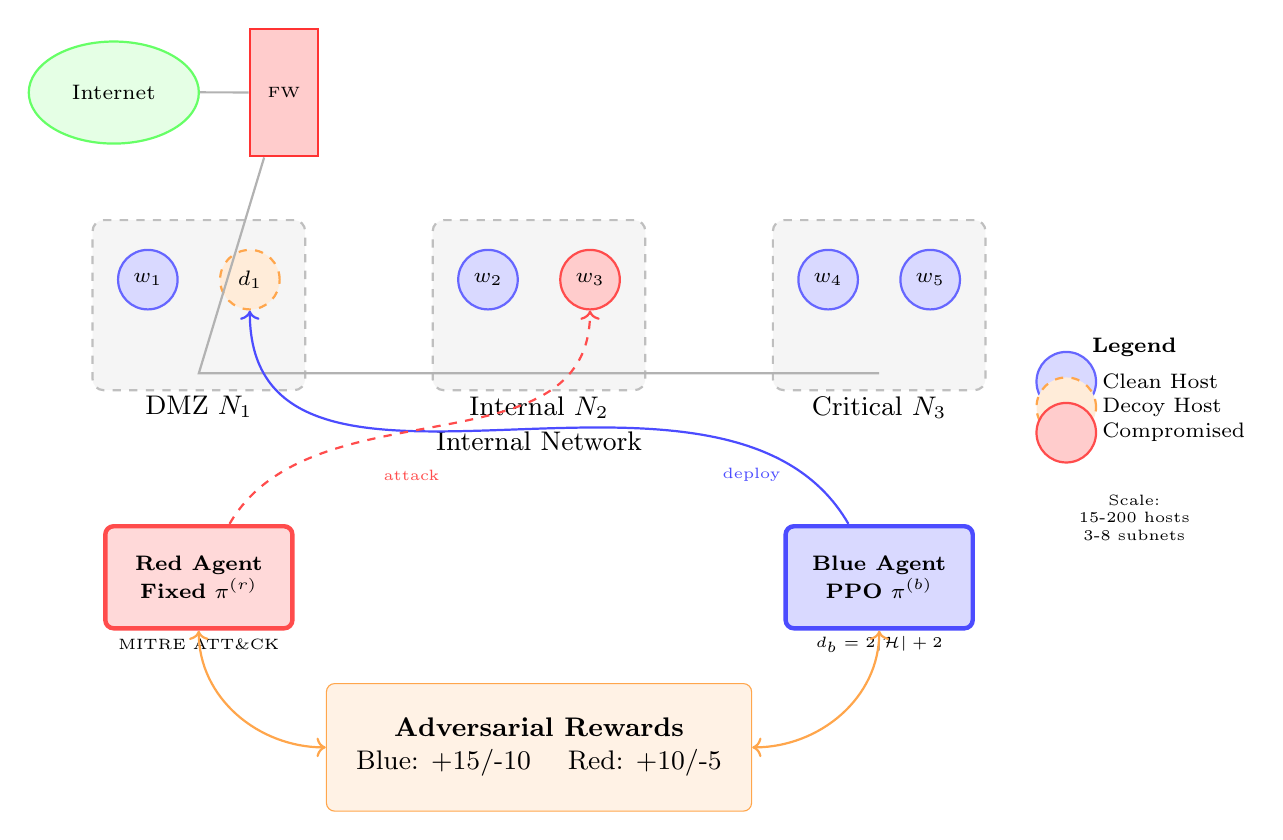
\begin{tikzpicture}[scale=1.08,transform shape,
    host/.style={circle, draw=blue!60, fill=blue!15, minimum size=7mm, font=\scriptsize, thick},
    decoy/.style={circle, draw=orange!70, fill=orange!15, minimum size=7mm, font=\scriptsize, thick, dashed},
    compromised/.style={circle, draw=red!70, fill=red!20, minimum size=7mm, font=\scriptsize, thick},
    subnet/.style={rectangle, draw=gray!50, fill=gray!8, minimum width=25mm, minimum height=20mm, thick, rounded corners=4pt, dashed},
    agentRed/.style={rectangle, draw=red!70, fill=red!15, minimum width=22mm, minimum height=12mm, font=\scriptsize, ultra thick, rounded corners=3pt},
    agentBlue/.style={rectangle, draw=blue!70, fill=blue!15, minimum width=22mm, minimum height=12mm, font=\scriptsize, ultra thick, rounded corners=3pt},
    firewall/.style={rectangle, draw=red!80, fill=red!20, minimum width=8mm, minimum height=15mm, font=\tiny, thick},
    internet/.style={ellipse, draw=green!60, fill=green!10, minimum width=20mm, minimum height=12mm, thick, align=center, font=\scriptsize}
]

% Internet - top left
\node[internet] (internet) at (-6, 6.5) {Internet};

% Firewall
\node[firewall] (firewall) at (-4, 6.5) {FW};

% Subnets - better spacing to avoid overlaps
\node[subnet] (subnet1) at (-5, 4) {};
\node[subnet] (subnet2) at (-1, 4) {};
\node[subnet] (subnet3) at (3, 4) {};

% Subnet labels - positioned clearly below subnets
\node[font=\small] at (-5, 2.8) {DMZ $N_1$};
\node[font=\small] at (-1, 2.8) {Internal $N_2$};
\node[font=\small] at (3, 2.8) {Critical $N_3$};

% Hosts - properly positioned within subnets
\node[host] (h1) at (-5.6, 4.3) {$w_1$};
\node[decoy] (d1) at (-4.4, 4.3) {$d_1$};

\node[host] (h2) at (-1.6, 4.3) {$w_2$};
\node[compromised] (h3) at (-0.4, 4.3) {$w_3$};

\node[host] (h4) at (2.4, 4.3) {$w_4$};
\node[host] (h5) at (3.6, 4.3) {$w_5$};

% Network backbone - adjusted positioning
\draw[thick, gray!60] (internet) -- (firewall);
\draw[thick, gray!60] (firewall) -- (-5, 3.2) -- (-1, 3.2) -- (3, 3.2);

% Internal Network label - positioned to avoid subnet overlap
\node[font=\small] at (-1, 2.4) {Internal Network};

% Agents - positioned lower to avoid overlap
\node[agentRed, align=center] (red) at (-5, 0.8) {\textbf{Red Agent}\\\textbf{Fixed} $\pi^{(r)}$};
\node[agentBlue, align=center] (blue) at (3, 0.8) {\textbf{Blue Agent}\\\textbf{PPO} $\pi^{(b)}$};

% Interactions with better label positioning
\draw[->, thick, blue!70] (blue) to[out=120, in=270] (d1);
\node[font=\tiny, blue!70] at (1.5, 2) {deploy};

\draw[->, thick, red!70, dashed] (red) to[out=60, in=270] (h3);
\node[font=\tiny, red!70] at (-2.5, 2) {attack};

% Essential state info
\node[font=\tiny] at (-5, 0.01) {MITRE ATT\&CK};
\node[font=\tiny] at (3, 0.01) {$d_b = 2|\mathcal{H}| + 2$};

% Rewards - positioned lower
\node[rectangle, draw=orange!70, fill=orange!10, minimum width=50mm, minimum height=15mm, rounded corners=3pt] (reward) at (-1, -1.2) {};
\node[font=\small, align=center] at (reward.center) {\textbf{Adversarial Rewards}\\Blue: +15/-10 \quad Red: +10/-5};

% Reward arrows
\draw[<->, orange!70, thick] (red.south) to[out=270, in=180] (reward.west);
\draw[<->, orange!70, thick] (blue.south) to[out=270, in=0] (reward.east);

\node[font=\scriptsize] at (6, 3.5) {\textbf{Legend}};
\node[host] at (5.2, 3.1) {}; \node[right, font=\scriptsize] at (5.5, 3.1) {Clean Host};
\node[decoy] at (5.2, 2.8) {}; \node[right, font=\scriptsize] at (5.5, 2.8) {Decoy Host};
\node[compromised] at (5.2, 2.5) {}; \node[right, font=\scriptsize] at (5.5, 2.5) {Compromised};

% Environment scale
\node[font=\tiny, align=center] at (6, 1.5) {Scale:\\15-200 hosts\\3-8 subnets};

\end{tikzpicture}
\end{adjustbox}
\end{center}
\vspace{-2mm}
\end{frame}

%----------------------------------------------------------------------
% PPO ARCHITECTURE - EXACT TIKZ FROM ORIGINAL
%----------------------------------------------------------------------
\begin{frame}{PPO Training Architecture}
\begin{center}
\scalebox{0.8}{
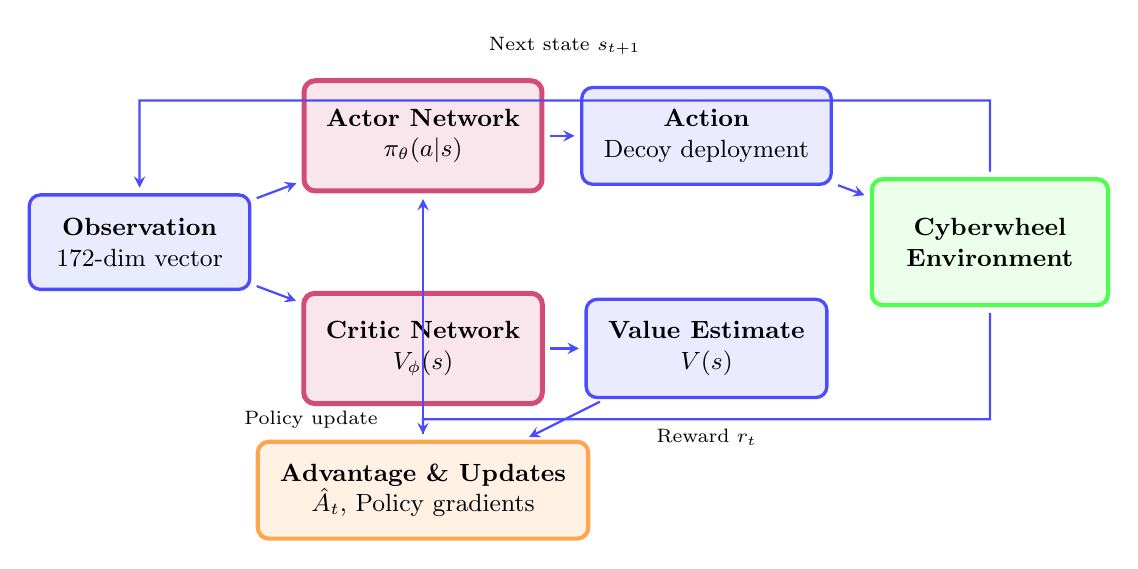
\begin{tikzpicture}[
    node distance=3cm,
    main/.style={draw=blue!70, rounded corners=4pt, fill=blue!8, 
                 inner sep=8pt, minimum width=2.8cm, minimum height=1.2cm, 
                 align=center, font=\small, line width=1.2pt},
    network/.style={draw=purple!70, rounded corners=4pt, fill=purple!10, 
                   inner sep=8pt, minimum width=2.8cm, minimum height=1.4cm, 
                   align=center, font=\small, line width=1.8pt},
    env/.style={draw=green!70, rounded corners=4pt, fill=green!8, 
               inner sep=8pt, minimum width=3cm, minimum height=1.6cm, 
               align=center, font=\small, line width=1.5pt},
    reward/.style={draw=orange!70, rounded corners=4pt, fill=orange!10, 
                   inner sep=8pt, minimum width=3.2cm, minimum height=1.2cm, 
                   align=center, font=\small, line width=1.5pt},
    flow/.style={-stealth, thick, blue!70, shorten >=2pt, shorten <=2pt},
    scale=0.9
]

% Left column: Input
\node[main] (obs) at (0,0) {
    \textbf{Observation}\\
    172-dim vector
};

% Center column: Networks
\node[network] (actor) at (4,1.5) {
    \textbf{Actor Network}\\
    $\pi_\theta(a|s)$
};

\node[network] (critic) at (4,-1.5) {
    \textbf{Critic Network}\\
    $V_\phi(s)$
};

% Right column: Outputs and Environment
\node[main] (action) at (8,1.5) {
    \textbf{Action}\\
    Decoy deployment
};

\node[main] (value) at (8,-1.5) {
    \textbf{Value Estimate}\\
    $V(s)$
};

\node[env] (environment) at (12,0) {
    \textbf{Cyberwheel}\\
    \textbf{Environment}
};

% Bottom: Learning components
\node[reward] (advantage) at (4,-3.5) {
    \textbf{Advantage \& Updates}\\
    $\hat{A}_t$, Policy gradients
};

% Forward flows (left to right, no crossing)
\draw[flow] (obs) -- (actor);
\draw[flow] (obs) -- (critic);
\draw[flow] (actor) -- (action);
\draw[flow] (critic) -- (value);
\draw[flow] (action) -- (environment);

% Feedback flows (right to left, separated levels)
\draw[flow] (environment) -- ++(0,2) -- ++(-12,0) -- (obs);
\node[above, font=\scriptsize] at (6,2.5) {Next state $s_{t+1}$};

\draw[flow] (environment) -- ++(0,-2.5) -- ++(-8,0) -- (advantage);
\node[below, font=\scriptsize] at (8,-2.5) {Reward $r_t$};

\draw[flow] (value) -- (advantage);

% Update flow (bottom to top, no crossing)
\draw[flow] (advantage) -- (actor);
\node[left, font=\scriptsize] at (3.5,-2.5) {Policy update};

\end{tikzpicture}
}
\end{center}

\begin{block}{Key Features}
\begin{itemize}
\item \textbf{172-dimensional observation space}: Alert history + network state + metadata  
\item \textbf{Actor-critic framework}: Stable policy optimization with value function guidance
\item \textbf{Strategic reward feedback}: Learn optimal deception placement through experience
\end{itemize}
\end{block}
\end{frame}

% ---------------------------------------------------------------------
% NEW SLIDE: RL Foundations (PPO math)
% ---------------------------------------------------------------------
\begin{frame}{RL Foundations (PPO — concise)}
\scriptsize
\begin{align*}
  &\pi_\theta(a|s)\quad\text{(actor / policy)}\\
  &V_\phi(s)\quad\text{(critic / value)}\\[4pt]
  &r_t(\theta)=\frac{\pi_\theta(a_t|s_t)}{\pi_{\theta_{\text{old}}}(a_t|s_t)}\\[2pt]
  &L^{\mathrm{CLIP}}(\theta)=\mathbb{E}_t\Big[\min\big(r_t(\theta)\,\hat A_t,\ \mathrm{clip}(r_t(\theta),1-\epsilon,1+\epsilon)\,\hat A_t\big)\Big]\\[6pt]
  &L(\theta,\phi)= -L^{\mathrm{CLIP}}(\theta) \;+\; c_1\,(V_\phi(s_t)-R_t)^2 \;-\; c_2\,\mathcal H(\pi_\theta)\\[6pt]
  &\text{GAE (compact): }\quad \hat A_t=\sum_{l=0}^{k-1}(\gamma\lambda)^l\delta_{t+l},\qquad 
  \delta_t=r_t+\gamma V_\phi(s_{t+1})-V_\phi(s_t)
\end{align*}

\vspace{4pt}
\small Notes: clipping stabilises policy updates; value loss (c1) and entropy regulariser (c2) improve convergence.
\end{frame}

%----------------------------------------------------------------------
% EXPERIMENTAL RESULTS
%----------------------------------------------------------------------
\begin{frame}{Key Results: 89\% Performance Improvement}
\begin{columns}[c]
\column{0.45\textwidth}
\textbf{\textcolor{ImperialBlue}{Algorithm Performance:}}

\centering
\begin{tabular}{|l|c|}
\hline
\rowcolor{ImperialLightBlue}
\textbf{Algorithm} & \textbf{Reward} \\
\hline
\rowcolor{green!20}
\textbf{PPO (Ours)} & \textbf{309.14} \\
Static Baseline & 163.81 \\
Rule Baseline & 79.16 \\
Inactive & -1.61 \\
\hline
\end{tabular}


\column{0.55\textwidth}
\textbf{\textcolor{cwAlert}{Security Effectiveness:}}
\begin{itemize}
    \item \textbf{\textcolor{cwAlert}{89\% improvement}} over static baseline
    \item \textbf{73.2\% deception success} rate (vs 45.1\% static)
    \item \textbf{82.4\% asset protection} rate (vs 61.7\% static)
    \item \textbf{2.3 timestep} detection latency (vs 4.1 static)
    \item \textbf{92.3\% correlation} with MITRE ATT\&CK patterns
    \item \textbf{84.8\% defense success} against real attacks
\end{itemize}
\end{columns}

\vspace{0.3cm}
\begin{exampleblock}{Statistical Validation}
\textbf{ANOVA p < 0.001}, Cohen's d > 0.8, 95\% confidence intervals, 5-seed validation
\end{exampleblock}
\end{frame}

%----------------------------------------------------------------------
% STRATEGIC BEHAVIORS
%----------------------------------------------------------------------
\begin{frame}{Learned Strategic Behaviors}
\begin{columns}[c]
\column{0.6\textwidth}
\textbf{\textcolor{ImperialBlue}{Emergent Intelligence:}}
\begin{itemize}
    \item \textbf{Balanced Strategy}: 20.4\% deploy, 19.2\% remove, 60.4\% wait
    \item \textbf{Learned Restraint}: Avoids over-deployment traps
    \item \textbf{Superior Consistency}: $\sigma = 37.37$ vs baseline variance
    \item \textbf{Adaptive Timing}: Strategic waiting periods
\end{itemize}

\textbf{\textcolor{cwDecoy}{Strategic Insights:}}
\begin{itemize}
    \item Agent learns \textbf{when NOT to act} (patience)
    \item Balances resource costs vs security benefits
    \item Adapts to attacker patterns without explicit programming
\end{itemize}

\column{0.4\textwidth}
\begin{center}
% Clean, self-contained pie chart. Wait leader forced straight down.
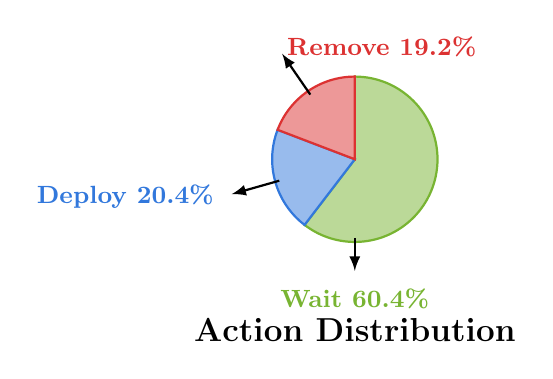
\begin{tikzpicture}[scale=1.0]
    \def\radius{1.05}
    % Percent -> angles (degrees)
    \def\angW{217.44} % Wait (60.4%)
    \def\angD{73.44}  % Deploy (20.4%)
    \def\angR{69.12}  % Remove (19.2%)
    \def\start{90}

    % slice boundary angles (clockwise)
    \pgfmathsetmacro{\aWend}{\start-\angW}
    \pgfmathsetmacro{\aDend}{\aWend-\angD}
    \pgfmathsetmacro{\aRend}{\aDend-\angR}

    % draw slices
    \draw[fill=cwDecoy!50, draw=cwDecoy, thick] (0,0) -- (\start:\radius) arc (\start:\aWend:\radius) -- cycle; % Wait
    \draw[fill=cwFlow!50,  draw=cwFlow,  thick] (0,0) -- (\aWend:\radius) arc (\aWend:\aDend:\radius) -- cycle; % Deploy
    \draw[fill=cwAlert!50, draw=cwAlert, thick] (0,0) -- (\aDend:\radius) arc (\aDend:\aRend:\radius) -- cycle; % Remove

    % mid angles for leader lines
    \pgfmathsetmacro{\midD}{\aWend-0.5*\angD}
    \pgfmathsetmacro{\midR}{\aDend-0.5*\angR}

    % Deploy label (left side)
    \draw[-{latex[length=2mm,width=2mm]}, thick] ({\midD}:{\radius*0.95}) -- ({\midD}:{\radius*1.55});
    \node[font=\bfseries\small, text=cwFlow, anchor=east] at ({\midD}:{\radius*1.65}) {Deploy 20.4\%};

    % Remove label (right side)
    \draw[-{latex[length=2mm,width=2mm]}, thick] ({\midR}:{\radius*0.95}) -- ({\midR}:{\radius*1.55});
    \node[font=\bfseries\small, text=cwAlert, anchor=west] at ({\midR}:{\radius*1.65}) {Remove 19.2\%};

    % Wait: force leader straight down and label directly below center
    \draw[-{latex[length=2mm,width=2mm]}, thick] (0,{\radius*0.95*-1}) -- (0,{-\radius*1.35});
    \node[font=\bfseries\small, text=cwDecoy, anchor=north] at (0,{-\radius*1.45}) {Wait 60.4\%};

    % Title under chart
    \node[below,font=\bfseries\large] at (0,-1.9) {Action Distribution};
\end{tikzpicture}
\end{center}
\end{columns}
\end{frame}

%----------------------------------------------------------------------
% SCALABILITY ANALYSIS
%----------------------------------------------------------------------
\begin{frame}{Scalability Analysis}
\begin{columns}[c]
\column{0.5\textwidth}
\textbf{\textcolor{ImperialBlue}{Network Size Performance:}}

\begin{center}
\begin{tabular}{|l|c|c|}
\hline
\rowcolor{ImperialLightBlue}
\textbf{Hosts} & \textbf{Reward} & \textbf{Time} \\
\hline
15 & 309.14 & 2.5h \\
50 & 325.42 & 6.2h \\
200 & 298.17 & 18.4h \\
\hline
\end{tabular}
\end{center}

\textbf{\textcolor{cwDecoy}{Scalability Properties:}}
\begin{itemize}
    \item \textbf{Consistent Performance}: 298-325 reward range
    \item \textbf{Sub-quadratic scaling}: O(n log n) complexity
    \item \textbf{Linear memory usage}: Practical for enterprise
    \item \textbf{Strategic consistency}: Behaviors stable across scales
\end{itemize}

\column{0.5\textwidth}
%\begin{center}
\textbf{Performance vs Network Size}

%\begin{tikzpicture}[scale=0.8]
%    \draw[->] (0,0) -- (4,0) node[right] {Network Size};
%    \draw[->] (0,0) -- (0,3) node[above] {Reward};
\begin{center}
\begin{tikzpicture}
\begin{axis}[
    width=7cm,
    height=4.5cm,
    xlabel={Network Size},
    ylabel={Reward},
    xlabel style={yshift=-0.3cm},
    ylabel style={yshift=0.2cm},
    xmin=0, xmax=220,
    ymin=288, ymax=344,
    xtick={15,50,200},
    xticklabel style={font=\scriptsize},
    ytick={298,309,325,339},
    yticklabel style={font=\scriptsize},
    grid=major,
    grid style={line width=.1pt, draw=gray!30},
    axis background/.style={fill=white},
]
\addplot[thick, draw=ImperialBlue, mark=*, mark options={fill=ImperialBlue}] coordinates {
    (15,309.14)
    (50,325.42)
    (200,298.17)
};
\addplot[dashed, red!60] coordinates {(15,309.14) (200,298.17)};
\end{axis}
\end{tikzpicture}
\end{center}

\textbf{\textcolor{cwAlert}{Enterprise Ready:}} Validated up to 200 hosts with maintained effectiveness
\end{columns}
\end{frame}

%----------------------------------------------------------------------
% REAL-WORLD VALIDATION
%----------------------------------------------------------------------
\begin{frame}{Real-World Validation}
\begin{columns}[c]
\column{0.5\textwidth}
\textbf{\textcolor{ImperialBlue}{MITRE ATT\&CK Integration:}}
\begin{itemize}
    \item \textbf{295 attack techniques} implemented
    \item \textbf{92.3\% behavioral correlation} with real patterns
    \item \textbf{Complete kill chain} coverage (4 phases)
    \item \textbf{Atomic Red Team} validation
\end{itemize}

\textbf{\textcolor{cwDecoy}{Attack Defense Success:}}
\begin{itemize}
    \item \textbf{84.8\% success rate} against real attack commands
    \item \textbf{Early disruption}: 2.3 timestep detection
    \item \textbf{Proactive defense}: Uncertainty creation vs reactive response
\end{itemize}

\column{0.5\textwidth}
\begin{center}
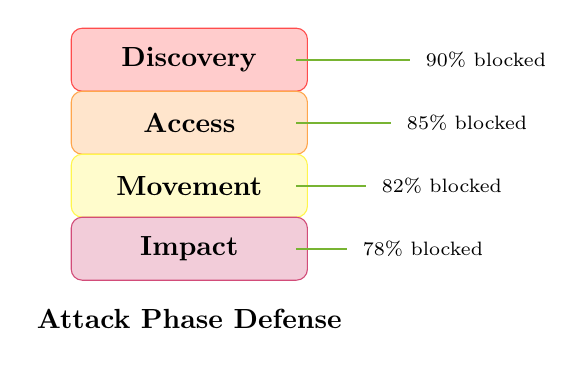
\begin{tikzpicture}[scale=0.8]
    % MITRE ATT&CK phases
    \node[draw=red!70, fill=red!20, rounded corners, minimum width=3cm, minimum height=0.8cm] at (0,3) {\textbf{Discovery}};
    \node[draw=orange!70, fill=orange!20, rounded corners, minimum width=3cm, minimum height=0.8cm] at (0,2) {\textbf{Access}};
    \node[draw=yellow!70, fill=yellow!20, rounded corners, minimum width=3cm, minimum height=0.8cm] at (0,1) {\textbf{Movement}};
    \node[draw=purple!70, fill=purple!20, rounded corners, minimum width=3cm, minimum height=0.8cm] at (0,0) {\textbf{Impact}};
    
    % Defense effectiveness
    \draw[thick, cwDecoy] (1.7,3) -- (3.5,3);
    \draw[thick, cwDecoy] (1.7,2) -- (3.2,2);
    \draw[thick, cwDecoy] (1.7,1) -- (2.8,1);
    \draw[thick, cwDecoy] (1.7,0) -- (2.5,0);
    
    \node[right] at (3.6,3) {\scriptsize 90\% blocked};
    \node[right] at (3.3,2) {\scriptsize 85\% blocked};
    \node[right] at (2.9,1) {\scriptsize 82\% blocked};
    \node[right] at (2.6,0) {\scriptsize 78\% blocked};
    
    \node[below] at (0,-0.8) {\textbf{Attack Phase Defense}};
\end{tikzpicture}
\end{center}
\end{columns}

\vspace{0.3cm}
\begin{alertblock}{Practical Deployment Ready}
\textbf{Enterprise-scale validation} with realistic attack patterns and \textbf{consistent cross-scale performance}
\end{alertblock}
\end{frame}

%----------------------------------------------------------------------
% METHODOLOGY
%----------------------------------------------------------------------
\begin{frame}{Research Methodology}
\begin{columns}[c]
\column{0.5\textwidth}
\textbf{\textcolor{ImperialBlue}{Experimental Framework:}}
\begin{itemize}
    \item \textbf{Multi-Agent Setup}: Learning blue vs fixed red (295 techniques)
    \item \textbf{Networks}: 15-200 hosts, realistic enterprise topologies
    \item \textbf{Training}: 10M timesteps, 5 random seeds
    \item \textbf{Baselines}: Static, Rule-based, Random, Inactive
\end{itemize}

\textbf{\textcolor{cwDecoy}{Statistical Rigor:}}
\begin{itemize}
    \item \textbf{ANOVA}: p < 0.001 significance
    \item \textbf{Effect Size}: Cohen's d > 0.8 (large)
    \item \textbf{Confidence}: 95\% intervals
    \item \textbf{Reproducibility}: 5-seed validation
\end{itemize}

\column{0.5\textwidth}
\textbf{\textcolor{cwAlert}{Novel Contributions:}}
\begin{enumerate}
    \item \textbf{First systematic PPO validation} for cyber deception
    \item \textbf{Real-world MITRE integration} with 92.3\% fidelity
    \item \textbf{Scalability characterization} across enterprise networks
    \item \textbf{Strategic behavior analysis} revealing emergent intelligence
    \item \textbf{Reproducible methodology} with open protocols
\end{enumerate}

\textbf{\textcolor{ImperialBlue}{Research Questions Answered:}}
\begin{itemize}
    \item PPO effectively learns adaptive strategies
    \item 89\% improvement over traditional baselines
    \item Strategic behaviors emerge and scale robustly
\end{itemize}
\end{columns}
\end{frame}

%----------------------------------------------------------------------
% FUTURE WORK
%----------------------------------------------------------------------
\begin{frame}{Future Directions \& Impact}
\scriptsize
\setlength{\parskip}{0pt}
\setlength{\topsep}{0pt}
\begin{columns}[t]
  % use a wider left column so content fills the available space
  \column{0.62\textwidth}
  \textbf{Research Extensions:}
  \vspace{2pt}
  {\setlength{\parskip}{0pt}%
   \begin{itemize}
     \item Real-world deployment in operational environments
     \item Adversarial co-evolution with learning attackers (self-play)
     \item Multi-defender coordination across distributed networks
     \item Integration with existing security infrastructure (SIEM, EDR)
     \item Explainable AI for analyst understanding and trust
   \end{itemize}
  }

  \vspace{4pt}
  \textbf{Technical Advances:}
  \vspace{2pt}
  {\setlength{\parskip}{0pt}%
   \begin{itemize}
     \item Advanced reward shaping for complex scenarios
     \item Transfer learning across network topologies
     \item Real-time adaptation to novel attack patterns
   \end{itemize}
  }

  \column{0.38\textwidth}
  \begin{block}{Broader Impact}
  \tiny
  This work establishes reinforcement learning as a viable approach for automated cybersecurity defense with rigorous experimental validation.
  \end{block}

  \vspace{4pt}
  \begin{block}{Key Takeaways}
  \tiny
  \begin{itemize}
      \item AI successfully learns sophisticated adaptive defense strategies
      \item \textbf{89\% improvement} demonstrates clear superiority
      \item Strategic restraint emerges naturally without explicit programming
      \item Performance scales robustly to enterprise networks
      \item Real attack correlation validates deployment readiness
  \end{itemize}
  \end{block}
\end{columns}
\end{frame}




%----------------------------------------------------------------------
% CONCLUSIONS
%----------------------------------------------------------------------
\begin{frame}{Conclusions}
\begin{center}
{\Large\textbf{\textcolor{ImperialNavy}{Adaptive AI-Driven Cyber Defense Works}}}
\end{center}

\begin{columns}[c]
\column{0.33\textwidth}
\begin{block}{\textcolor{cwAlert}{Performance}}
\begin{center}
{\huge\textbf{89\%}}\\
\textbf{Improvement}\\
over static baselines
\end{center}
\end{block}

\column{0.33\textwidth}
\begin{block}{\textcolor{cwFlow}{Intelligence}}
\begin{center}
\textbf{Strategic}\\
\textbf{Behaviors}\\
emerge naturally
\end{center}
\end{block}

\column{0.33\textwidth}
\begin{block}{\textcolor{cwDecoy}{Scale}}
\begin{center}
\textbf{Enterprise}\\
\textbf{Ready}\\
15-200 hosts validated
\end{center}
\end{block}
\end{columns}

\vspace{0.5cm}

\begin{alertblock}{Research Impact}
\textbf{First rigorous validation} of reinforcement learning for cybersecurity deception with \textbf{real-world attack correlation} and \textbf{enterprise-scale deployment readiness}
\end{alertblock}

\vspace{0.3cm}
\begin{center}
\textcolor{ImperialBlue}{\textbf{Questions?}}\\
\textcolor{ImperialBlue}{miracle.akanmode24@imperial.ac.uk}
\end{center}
\end{frame}

\end{document}